% !TEX root = main.tex
\section{Introduction}
\label{sec:intro}



Enabling easy and efficient travel is the goal of many transit information technologies being developed today. Examples of information that these systems might provide include directions from one place to another\footnote{http://maps.google.com}, current traffic conditions\footnote{http://waze.com}, public transit arrival and departure times\footnote{http://onebusaway.org}, or wait time at the airport\footnote{http://gomiflight.com/}. Additionally, since technologies such as smartphones have become more ubiquitous, many applications are now drawing on contributions from travellers using these apps on-the-go to collect information that is localized, descriptive, and up-to-date \cite{harding-2013}. However, ensuring that these benefits are present means that information contributions must not only be accurate, but sustainable. This requires continuing participation from the community, whose motivations for contributing are diverse and may wane over time \cite{moore-2007}.

In this paper, we examine a particular transit information technology called StopInfo. StopInfo provides very detailed information about bus stops with the goal of helping public transit riders, particularly those with visual impairments, find and verify bus stop locations. Preliminary evaluations of StopInfo have shown that it supports independence of blind and low vision transit riders, who reported taking more transit trips with StopInfo than they might have without the tool \cite{campbell-2014}. 

The information presented in StopInfo comes from internal information from a transit agency in the Seattle area augmented with information that is entered by the community, primarily as individuals wait at transit stops. In its first year of deployment, StopInfo has received 1879 user submissions about 1148 unique bus stops in the Seattle area. Due in part to a number of press releases and community outreach events, participation has been relatively well sustained for the first twelve months of deployment. However, as might be expected, the number of new submissions has begun to decline (Figure \ref{fig:submissions}). In order to make sure information is accurate and up-to-date, it is important for StopInfo to support contributors' motivations for continuing to enter information, which may encourage increased or long term participation \cite{reed-2013}.

\begin{figure}[H]
\centering
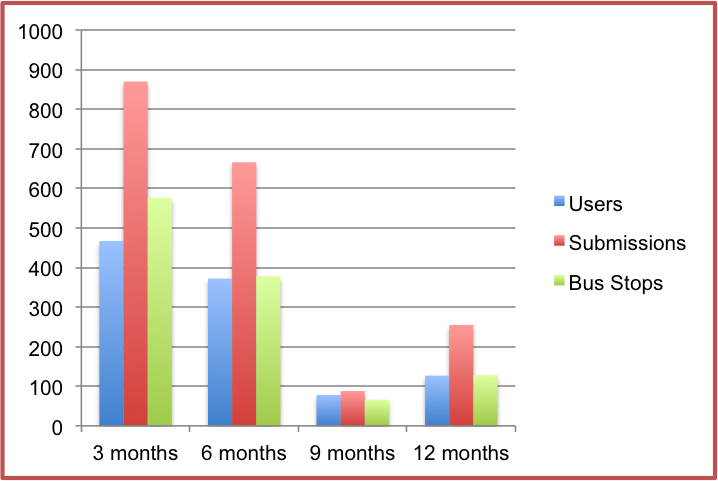
\includegraphics[width=.45\textwidth]{Chart2.png}
\caption{Submission numbers for StopInfo over the first twelve months of deployment. The chart shows the new users, information submissions, and bus stops for each three-month period. We had a major press release occur five months into deployment, and participated in outreach events for StopInfo ten months into deployment.}
\label{fig:submissions}
\end{figure} 


Toward this end, we employ theory and methodology from Value Sensitive Design \cite{friedman-amis-2006} to understand and elicit the values and motivations associated with contributing information about bus stops to StopInfo. In particular, we conduct a survey with previous contributors to the StopInfo system as well as non-contributors (i.e., people who have not contributed to StopInfo before and may or may not be willing to contribute in the future), and are in the process of conducting follow-up interviews with some of these individuals. Early survey and interview results inform us of possible system designs that can potentially help maintain the level of contributions from current StopInfo contributors as well as encourage non-contributors to participate. 




